\documentclass[]{article}
\usepackage{lmodern}
\usepackage{amssymb,amsmath}
\usepackage{ifxetex,ifluatex}
\usepackage{fixltx2e} % provides \textsubscript
\ifnum 0\ifxetex 1\fi\ifluatex 1\fi=0 % if pdftex
  \usepackage[T1]{fontenc}
  \usepackage[utf8]{inputenc}
\else % if luatex or xelatex
  \ifxetex
    \usepackage{mathspec}
  \else
    \usepackage{fontspec}
  \fi
  \defaultfontfeatures{Ligatures=TeX,Scale=MatchLowercase}
\fi
% use upquote if available, for straight quotes in verbatim environments
\IfFileExists{upquote.sty}{\usepackage{upquote}}{}
% use microtype if available
\IfFileExists{microtype.sty}{%
\usepackage{microtype}
\UseMicrotypeSet[protrusion]{basicmath} % disable protrusion for tt fonts
}{}
\usepackage{hyperref}
\hypersetup{unicode=true,
            pdfborder={0 0 0},
            breaklinks=true}
\urlstyle{same}  % don't use monospace font for urls
\usepackage{color}
\usepackage{fancyvrb}
\newcommand{\VerbBar}{|}
\newcommand{\VERB}{\Verb[commandchars=\\\{\}]}
\DefineVerbatimEnvironment{Highlighting}{Verbatim}{commandchars=\\\{\}}
% Add ',fontsize=\small' for more characters per line
\newenvironment{Shaded}{}{}
\newcommand{\KeywordTok}[1]{\textcolor[rgb]{0.00,0.44,0.13}{\textbf{{#1}}}}
\newcommand{\DataTypeTok}[1]{\textcolor[rgb]{0.56,0.13,0.00}{{#1}}}
\newcommand{\DecValTok}[1]{\textcolor[rgb]{0.25,0.63,0.44}{{#1}}}
\newcommand{\BaseNTok}[1]{\textcolor[rgb]{0.25,0.63,0.44}{{#1}}}
\newcommand{\FloatTok}[1]{\textcolor[rgb]{0.25,0.63,0.44}{{#1}}}
\newcommand{\ConstantTok}[1]{\textcolor[rgb]{0.53,0.00,0.00}{{#1}}}
\newcommand{\CharTok}[1]{\textcolor[rgb]{0.25,0.44,0.63}{{#1}}}
\newcommand{\SpecialCharTok}[1]{\textcolor[rgb]{0.25,0.44,0.63}{{#1}}}
\newcommand{\StringTok}[1]{\textcolor[rgb]{0.25,0.44,0.63}{{#1}}}
\newcommand{\VerbatimStringTok}[1]{\textcolor[rgb]{0.25,0.44,0.63}{{#1}}}
\newcommand{\SpecialStringTok}[1]{\textcolor[rgb]{0.73,0.40,0.53}{{#1}}}
\newcommand{\ImportTok}[1]{{#1}}
\newcommand{\CommentTok}[1]{\textcolor[rgb]{0.38,0.63,0.69}{\textit{{#1}}}}
\newcommand{\DocumentationTok}[1]{\textcolor[rgb]{0.73,0.13,0.13}{\textit{{#1}}}}
\newcommand{\AnnotationTok}[1]{\textcolor[rgb]{0.38,0.63,0.69}{\textbf{\textit{{#1}}}}}
\newcommand{\CommentVarTok}[1]{\textcolor[rgb]{0.38,0.63,0.69}{\textbf{\textit{{#1}}}}}
\newcommand{\OtherTok}[1]{\textcolor[rgb]{0.00,0.44,0.13}{{#1}}}
\newcommand{\FunctionTok}[1]{\textcolor[rgb]{0.02,0.16,0.49}{{#1}}}
\newcommand{\VariableTok}[1]{\textcolor[rgb]{0.10,0.09,0.49}{{#1}}}
\newcommand{\ControlFlowTok}[1]{\textcolor[rgb]{0.00,0.44,0.13}{\textbf{{#1}}}}
\newcommand{\OperatorTok}[1]{\textcolor[rgb]{0.40,0.40,0.40}{{#1}}}
\newcommand{\BuiltInTok}[1]{{#1}}
\newcommand{\ExtensionTok}[1]{{#1}}
\newcommand{\PreprocessorTok}[1]{\textcolor[rgb]{0.74,0.48,0.00}{{#1}}}
\newcommand{\AttributeTok}[1]{\textcolor[rgb]{0.49,0.56,0.16}{{#1}}}
\newcommand{\RegionMarkerTok}[1]{{#1}}
\newcommand{\InformationTok}[1]{\textcolor[rgb]{0.38,0.63,0.69}{\textbf{\textit{{#1}}}}}
\newcommand{\WarningTok}[1]{\textcolor[rgb]{0.38,0.63,0.69}{\textbf{\textit{{#1}}}}}
\newcommand{\AlertTok}[1]{\textcolor[rgb]{1.00,0.00,0.00}{\textbf{{#1}}}}
\newcommand{\ErrorTok}[1]{\textcolor[rgb]{1.00,0.00,0.00}{\textbf{{#1}}}}
\newcommand{\NormalTok}[1]{{#1}}
\usepackage{graphicx,grffile}
\makeatletter
\def\maxwidth{\ifdim\Gin@nat@width>\linewidth\linewidth\else\Gin@nat@width\fi}
\def\maxheight{\ifdim\Gin@nat@height>\textheight\textheight\else\Gin@nat@height\fi}
\makeatother
% Scale images if necessary, so that they will not overflow the page
% margins by default, and it is still possible to overwrite the defaults
% using explicit options in \includegraphics[width, height, ...]{}
\setkeys{Gin}{width=\maxwidth,height=\maxheight,keepaspectratio}
\IfFileExists{parskip.sty}{%
\usepackage{parskip}
}{% else
\setlength{\parindent}{0pt}
\setlength{\parskip}{6pt plus 2pt minus 1pt}
}
\setlength{\emergencystretch}{3em}  % prevent overfull lines
\providecommand{\tightlist}{%
  \setlength{\itemsep}{0pt}\setlength{\parskip}{0pt}}
\setcounter{secnumdepth}{0}
% Redefines (sub)paragraphs to behave more like sections
\ifx\paragraph\undefined\else
\let\oldparagraph\paragraph
\renewcommand{\paragraph}[1]{\oldparagraph{#1}\mbox{}}
\fi
\ifx\subparagraph\undefined\else
\let\oldsubparagraph\subparagraph
\renewcommand{\subparagraph}[1]{\oldsubparagraph{#1}\mbox{}}
\fi

\date{}

\begin{document}

\section{Networking}\label{networking}

Networking has become arguably the most important use of computers in
the past 10-20 years. Most of us nowadays can't stand a place without
wifi or any connectivity, so it is crucial as programmers that you have
an understanding of networking and how to program to communicate across
networks. Although it may sound complicated, POSIX has defined nice
standards that make connecting to the outside world easy. POSIX also
lets you peer underneath the hood and optimize all the little parts of
each connection to write high performant

\subsection{The OSI Model}\label{the-osi-model}

The Open Source Interconnection 7 layer model (OSI Model) is a sequence
of segments that define standards for both infrastructure and protocols
for forms of radio communication, in our case the internet. The 7 layer
model is as follows

\begin{enumerate}
\item
  Layer 1: The physical layer. These are the actual waves that carry the
  bauds across the wire. As an aside, bits don't cross the wire because
  in most mediums you can alter two characterstics of a wave -- the
  amplitude and the frequency -- and get more bits per clock cycle.
\item
  Layer 2: The link layer. This is how each of the agents react to
  certain events (error detection, noisy channels, etc). This is where
  Ethernet and WiFi live.
\item
  Layer 3: The network layer. This is the heart of the internet. The
  bottom two protocols deal with communication between two different
  computers that are directly connected. This layer deals with routing
  packets from one endpoint to another.
\item
  Layer 4: The transport layer. This layer specifies how the slices of
  data are received. The bottom three layers make no guarantee about the
  order that packets are received and what happens when a packet is
  dropped. Using different protocols, this layer can.
\item
  Layer 5: The session layer. This layer makes sure that if a connection
  in the previous layers is dropped, a new connection in the lower
  layers can be established, and it looks like a nothing happened to the
  end user.
\item
  Layer 6: The presentation layer. This layer deals with encryption,
  compression, and data translation. For example, portability between
  different operating systems like translating newlines to windows
  newlines.
\item
  Layer 7: The application layer. The application layer is where many
  different protocols live. HTTP and FTP are both defined at this level.
  This is typically where we define protocols across the internet. As
  programmers, we only go lower when we think we can create algorithms
  that are more suited to our needs than all of the below.
\end{enumerate}

Just to be clear this is not a networking class. We won't go over most
of these layers in depth. We will focus on some aspects of layers 3, 4,
and 7 because they are essential to know if you are going to be doing
something with the internet, which at some point in your career you will
be. As for another definition, a protocol is a set of specifications put
forward by the Internet Engineering Task Force that govern how
implementers of protocol have their program or circuit behave under
specific circumastnces.

\subsection{Layer 3: The Internet
Protocol}\label{layer-3-the-internet-protocol}

The following is the ``30 second'' introduction to internet protocol
(IP) - which is the primary way to send packets (``datagrams'') of
information from one machine to another. ``IP4'', or more precisely,
``IPv4'' is version 4 of the Internet Protocol that describes how to
send packets of information across a network from one machine to
another. Roughly 95\% of all packets on the Internet today are IPv4
packets. A significant limitation of IPv4 is that source and destination
addresses are limited to 32 bits. IPv4 was designed at a time when the
idea of 4 billion devices connected to the same network was unthinkable
- or at least not worth making the packet size larger. IPv4 address are
written typically in a sequence of four octets delimited by periods
``255.255.255.0'' for example.

Each IPv4 packet includes a very small header - typically 20 bytes (more
precisely, ``octets''), that includes a source and destination address.
Conceptually the source and destination addresses can be split into two:
a network number (the upper bits) and the lower bits represent a
particular host number on that network.

A newer packet protocol ``IPv6'' solves many of the limitations of IPv4
like making routing tables simpler and 128 bit addresses. However, less
than 5\% of web traffic is IPv6 based. We write IPv6 addresses in a
sequence of eight, four hexadecimal delimiters like
``1F45:0000:0000:0000:0000:0000:0000:0000''. Since that can get unruly,
we can omit the zeros ``1F45::''.

A machine can have an IPv6 address and an IPv4 address.

A special IPv4 address is \texttt{127.0.0.1}, IPv6 as
\texttt{0:0:0:0:0:0:0:1} or \texttt{::1} also known as localhost.
Packets sent to 127.0.0.1 will never leave the machine; the address is
specified to be the same machine.

\subsubsection{In-depth IPv4
Specification}\label{in-depth-ipv4-specification}

The internet protocol deals with routing, fragmentation, and reassembly
of datagram fragments. Datagrams are formatted as such

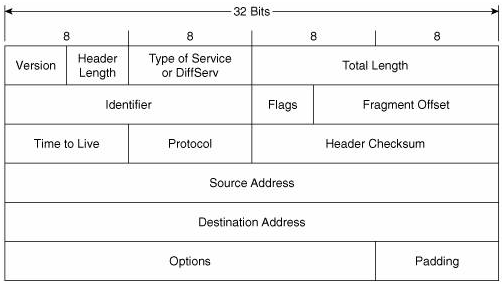
\includegraphics{networking/images/ipv4_header.png}

\begin{enumerate}
\item
  The first octet is the version number, either 4 or 6
\item
  The next octet is how long the header is. Although it may seem that
  the header is constant size, you can include optional parameters to
  augment the path taken or other instructions
\item
  The next two octets specify the total length of the datagram. This
  means this is the header, the data, footer, and padding. This is given
  in multiple of octets, meaning that a value of 20 means 20 octets.
\item
  The next two are Identification number. IP handles taking packets that
  are too big to be sent over the phsyical wire and chunks them up. As
  such, this number identifies what datagram this originally belonged
  to.
\item
  The next octet is various bit flags that can be set.
\item
  The next octet and half is fragment number. If this packet was
  fragmented, this is the number this fragment represents
\item
  The next octet is time to live. So this is the number of ``hops''
  (travels over a wire) a packet is allowed to go. This is set because
  different routing protocols could cuase packets to go in circles, the
  packets must be dropped at some point.
\item
  The next octet is the protocol number. Although protocols between
  different layers of the OCI model are supposed to be black boxes, this
  is included, so that hardware can peer into the underlying protocol
  efficiently. Take for example IP over IP (yes you can do that!). Your
  ISP wraps IPv4 packets sent from your computer to the ISP in another
  IP layer and sends the packet off to be delivered to the website. On
  the reverse trip the packet is ``unwrapped'' and the original IP
  datagram is sent to your computer. This was done because we ran out of
  IP addresses, and this adds additional overhead but it is a necessary
  fix. Other common protocols are TCP, UDP, etc.
\item
  The next two octets is an internet checksum. This is a CRC that is
  calculated to make sure that a wide variety of bit errors are
  detected.
\item
  Source address is what people generally refer to as the IP address.
  There is no verification of this, so one host can pretend to be any IP
  address possible
\item
  Destination address is where you want the packet to be sent to. This
  is crucial in the routing process as you need that to route.
\item
  After: Your data! All layer of higher order protocols are put in there
\item
  Additional options: Hosts of additional options
\item
  Footer: A bit of padding to make sure your data is a multiple of 8
\end{enumerate}

\subsubsection{Routing}\label{routing}

The internet protocol routing is an amazing intersection of theory and
application. We can imagine the entire internet as a set of graphs. Most
peers are connected to what we call ``peering points'' these are the
WIFI routers and the ethernet ports that one finds in their house, work,
or public. These peering points are then connected to a wired network of
routers, switches, and servers that all route themselves. At a top level
there are two types of routing

\begin{enumerate}
\item
  Internal Routing Protocols. Internal protocols is routing designed for
  within an ISP's network. These protocols are meant to be fast and more
  trusting because all computers, switches, and routers are part of an
  ISP. communication between two routers.
\item
  External Routing Protocols. These typically happen to be ISP to ISP
  protocol. Certain routers are designated as border routers. These
  routers talk to routers from ISPs have have different policies from
  accepting or receiving packets. If an evil ISP is trying to dump all
  network traffic onto your ISP, these routers would deal with that.
  These protocols also deal with gathering information about the outside
  world to each router. In most routing protocols using link state or
  OSPF, a router must necessarily calculate the shortest path to the
  destination. This means it needs information about the ``foreign''
  routers which is disseminated according to these protocols.
\end{enumerate}

These two protocols have to interplay with each other nicely in order to
make sure that packets are mostly delivered. In addition, ISPs need to
be nice to each other because theoretically an ISP can handle lower load
by forwarding all packets to another ISP. If everyone does that then, no
packets get delivered at all which won't make customers happy at all. So
these two protocols need to be fair so the end result works

If you want to read more about this, look at the wikipedia page for
routing here \href{https://en.wikipedia.org/wiki/Routing}{Routing}.

\subsubsection{Fragmentation/Reassembly}\label{fragmentationreassembly}

Lower layers like WiFi and Ethernet have maximum transmission sizes. The
reason being is

\begin{enumerate}
\item
  One host shouldn't crowd the medium for too long
\item
  If an error occurs, we want some sort of ``progress bar'' on how far
  the communication has gone instead of retransmitting the stream
\item
  There are physical limitations as well, keeping a laser beam in optics
  working continuously may cause bit errors.
\end{enumerate}

As such if the internet protocol receives a packet that is too big for
the maximum size, it must chunk it up. TCP calculates how many datagrams
it needs to construct a packet and ensures that they are all transmitted
and reconstructed at the end receiver. The reason that we barely use
this feature is that if any fragment is lost, the entire packet is lost.
Meaning that, assuming the probability of receiving a packet assuming
each fragment is lost with an independent percentage, the probability of
successfully sending a packet drops off exponentially as packet size
increases.

As such, TCP slices its packets so that it fits inside on IP datagram.
The only time that this applies is when sending UDP packets that are too
big, but most people who are using UDP optimize and set the same packet
size as well.

\subsubsection{IP Multicast}\label{ip-multicast}

A little known feature is that using the IP protocol one can send a
datagram to all devices connected to a router in what is called a
multicast. Multicasts can also be configured with groups, so one can
efficiently slice up all connected routers and send a piece of
information to all of them efficiently. To access this in a higher
protocol, you need to use UDP and specify a few more options. Note that
this will cause undo stress on the network, so a series of multicasts
could flood the network fast.

\subsubsection{What's the deal with
IPv6?}\label{whats-the-deal-with-ipv6}

One of the big features of IPv6 is the address space. The world ran out
of IP addresses a while ago and has been using hacks to get around that.
With IPv6 there are enough internal and external addresses, so that
unless we discover alien civilizations, we probably won't run out. The
other benefit is that these addresses are leased not bought, meaning
that if something drastic happens in let's say the internet of things
and there needs to be a change in the block addressing scheme, it can be
done.

Another big feature is security through IPsec. IPv4 was designed with
little to no security in mind. As such, now there is a key exchange
similar to TLS in higher layers that allows you to encrypt
communication.

Another feature is simplified processing. In order to make the internet
fast, IPv4 and IPv6 headers alike are actually implemented in hardware.
That means that all header options are processed in circuits as they
come in. The problem is that as the IPv4 spec grew to include a copious
amount of headers, the hardware had to become more and more advanced to
support those headers. IPv6 reorders the headers so that packets can be
dropped and routed with less hardware cycles. In the case of the
internet, every cycle matters when trying to route the world's traffic.

\subsubsection{getnameinfo Example: What's my IP
address?}\label{getnameinfo-example-whats-my-ip-address}

To obtain a linked list of IP addresses of the current machine use
\texttt{getifaddrs} which will return a linked list of IPv4 and IPv6 IP
addresses (and potentially other interfaces too). We can examine each
entry and use \texttt{getnameinfo} to print the host's IP address. The
ifaddrs struct includes the family but does not include the sizeof the
struct. Therefore we need to manually determine the struct sized based
on the family (IPv4 v IPv6)

\begin{Shaded}
\begin{Highlighting}[]
 \NormalTok{(family == AF_INET) ? }\KeywordTok{sizeof}\NormalTok{(}\KeywordTok{struct} \NormalTok{sockaddr_in) : }\KeywordTok{sizeof}\NormalTok{(}\KeywordTok{struct} \NormalTok{sockaddr_in6)}
\end{Highlighting}
\end{Shaded}

The complete code is shown below.

\begin{Shaded}
\begin{Highlighting}[]
    \DataTypeTok{int} \NormalTok{required_family = AF_INET; }\CommentTok{// Change to AF_INET6 for IPv6}
    \KeywordTok{struct} \NormalTok{ifaddrs *myaddrs, *ifa;}
    \NormalTok{getifaddrs(&myaddrs);}
    \DataTypeTok{char} \NormalTok{host[}\DecValTok{256}\NormalTok{], port[}\DecValTok{256}\NormalTok{];}
    \KeywordTok{for} \NormalTok{(ifa = myaddrs; ifa != NULL; ifa = ifa->ifa_next) \{}
        \DataTypeTok{int} \NormalTok{family = ifa->ifa_addr->sa_family;}
        \KeywordTok{if} \NormalTok{(family == required_family && ifa->ifa_addr) \{}
            \KeywordTok{if} \NormalTok{(}\DecValTok{0} \NormalTok{== getnameinfo(ifa->ifa_addr,}
                                \NormalTok{(family == AF_INET) ? }\KeywordTok{sizeof}\NormalTok{(}\KeywordTok{struct} \NormalTok{sockaddr_in) :}
                                \KeywordTok{sizeof}\NormalTok{(}\KeywordTok{struct} \NormalTok{sockaddr_in6),}
                                \NormalTok{host, }\KeywordTok{sizeof}\NormalTok{(host), port, }\KeywordTok{sizeof}\NormalTok{(port)}
                                 \NormalTok{, NI_NUMERICHOST | NI_NUMERICSERV  ))}
                \NormalTok{puts(host);}
            \NormalTok{\}}
        \NormalTok{\}}
\end{Highlighting}
\end{Shaded}

\subsubsection{IP Address, Shell
Version}\label{whats-my-machines-ip-address-shell-version}

Answer: use \texttt{ifconfig} (or Windows's ipconfig) However this
command generates a lot of output for each interface, so we can filter
the output using grep

\begin{verbatim}
ifconfig | grep inet

Example output:
    inet6 fe80::1%lo0 prefixlen 64 scopeid 0x1 
    inet 127.0.0.1 netmask 0xff000000 
    inet6 ::1 prefixlen 128 
    inet6 fe80::7256:81ff:fe9a:9141%en1 prefixlen 64 scopeid 0x5 
    inet 192.168.1.100 netmask 0xffffff00 broadcast 192.168.1.255
\end{verbatim}

\subsubsection{How do I use getaddrinfo to convert the hostname into an
IP
address?}\label{how-do-i-use-getaddrinfo-to-convert-the-hostname-into-an-ip-address}

The function \texttt{getaddrinfo} can convert a human readable domain
name (e.g. \texttt{www.illinois.edu}) into an IPv4 and IPv6 address. In
fact it will return a linked-list of addrinfo structs:

\begin{Shaded}
\begin{Highlighting}[]
\KeywordTok{struct} \NormalTok{addrinfo \{}
    \DataTypeTok{int}              \NormalTok{ai_flags;}
    \DataTypeTok{int}              \NormalTok{ai_family;}
    \DataTypeTok{int}              \NormalTok{ai_socktype;}
    \DataTypeTok{int}              \NormalTok{ai_protocol;}
    \NormalTok{socklen_t        ai_addrlen;}
    \KeywordTok{struct} \NormalTok{sockaddr *ai_addr;}
    \DataTypeTok{char}            \NormalTok{*ai_canonname;}
    \KeywordTok{struct} \NormalTok{addrinfo *ai_next;}
\NormalTok{\};}
\end{Highlighting}
\end{Shaded}

It's very easy to use. For example, suppose you wanted to find out the
numeric IPv4 address of a webserver at www.bbc.com. We do this in two
stages. First use getaddrinfo to build a linked-list of possible
connections. Secondly use \texttt{getnameinfo} to convert the binary
address into a readable form.

\begin{Shaded}
\begin{Highlighting}[]
\OtherTok{#include <stdio.h>}
\OtherTok{#include <stdlib.h>}
\OtherTok{#include <sys/types.h>}
\OtherTok{#include <sys/socket.h>}
\OtherTok{#include <netdb.h>}

\KeywordTok{struct} \NormalTok{addrinfo hints, *infoptr; }\CommentTok{// So no need to use memset global variables}

\DataTypeTok{int} \NormalTok{main() \{}
  \NormalTok{hints.ai_family = AF_INET; }\CommentTok{// AF_INET means IPv4 only addresses}

  \DataTypeTok{int} \NormalTok{result = getaddrinfo(}\StringTok{"www.bbc.com"}\NormalTok{, NULL, &hints, &infoptr);}
  \KeywordTok{if} \NormalTok{(result) \{}
    \NormalTok{fprintf(stderr, }\StringTok{"getaddrinfo: %s}\CharTok{\textbackslash{}n}\StringTok{"}\NormalTok{, gai_strerror(result));}
    \NormalTok{exit(}\DecValTok{1}\NormalTok{);}
  \NormalTok{\}}

  \KeywordTok{struct} \NormalTok{addrinfo *p;}
  \DataTypeTok{char} \NormalTok{host[}\DecValTok{256}\NormalTok{];}

  \KeywordTok{for}\NormalTok{(p = infoptr; p != NULL; p = p->ai_next) \{}

    \NormalTok{getnameinfo(p->ai_addr, p->ai_addrlen, host, }\KeywordTok{sizeof}\NormalTok{(host), NULL, }\DecValTok{0}\NormalTok{, NI_NUMERICHOST);}
    \NormalTok{puts(host);}
  \NormalTok{\}}

  \NormalTok{freeaddrinfo(infoptr);}
  \KeywordTok{return} \DecValTok{0}\NormalTok{;}
\NormalTok{\}}
\end{Highlighting}
\end{Shaded}

Typical output:

\begin{verbatim}
212.58.244.70
212.58.244.71
\end{verbatim}

If you are wondering how the the computer maps hostnames to addresses,
we will talk about that in Layer 7. Spoiler: It is a service called DNS

\subsubsection{What is a port?}\label{what-is-a-port}

A port is actually not a part of the IP protocol. IP packets are sent to
addresses, but we frequently see IP addresses linked with ports. Ports
help higher order protocols multiplexes multiple clients sending packets
to the same IP address.

A process can listen for incoming packets on a particular port. However
only processes with super-user (root) access can listen on ports
\textless{} 1024. Any process can listen on ports 1024 or higher. An
often used port is port 80: Port 80 is used for unencrypted http
requests (i.e.~web pages). For example, if a web browser connects to
http://www.bbc.com/, then it will be connecting to port 80.

\subsection{Layer 4: TCP and Client}\label{layer-4-tcp-and-client}

\subsubsection{What is TCP? When is it
used?}\label{what-is-tcp-when-is-it-used}

TCP is a connection-based protocol that is built on top of IPv4 and IPv6
(and therefore can be described as ``TCP/IP'' or ``TCP over IP''). TCP
creates a \emph{pipe} between two machines and abstracts away the low
level packet-nature of the Internet: Thus, under most conditions, bytes
sent from one machine will eventually arrive at the other end without
duplication or data loss.

TCP will automatically manage resending packets, ignoring duplicate
packets, re-arranging out-of-order packets and changing the rate at
which packets are sent.

TCP's three way handshake is known as SYN, SYN-ACK, and ACK. The diagram
on this page helps with understanding the TCP handshake.
\href{http://www.inetdaemon.com/tutorials/internet/tcp/3-way_handshake.shtml}{TCP
Handshake}

Most services on the Internet today (e.g.~a web service) use TCP because
it hides the complexity of lower, packet-level nature of the Internet.

\subsubsection{TCP In Depth}\label{tcp-in-depth}

TCP has a number of features that set it apart from the other transport
protocol UDP.

\begin{enumerate}
\item
  Ports. With IP, you are only allowed to send packets to a machine. If
  you want one machine to handle multiple flows of data, you have to do
  it manually with IP. TCP abstracts that an gives the programmer a set
  of virtual sockets. Clients specify the socket that you want the
  packet sent to and the TCP protocol makes sure that applications that
  are waiting for packets on that port receive that.
\item
  Retransmission. Packets can get dropped due to network errors or
  congestion. As such, they need to be retransmitted but at the same
  time the retransmission shouldn't cause packets more packets to be
  dropped. This needs to balance the tradeoff between flooding the
  network and speed.
\item
  Out of order packets. Packets may get routed more favorably due to
  various reasons in IP. If a later packet arrives before another
  packet, the protocol should detect and reorder them.
\item
  Duplicate packets. Packets can arrive twice. Packets can arrive twice.
  As such, a protocol need to be able to differentiate between two
  packets given a sequence number subject to overflow.
\item
  Error correction. There is a TCP checksum that handles bit errors.
  This is rarely used though.
\item
  Flow Control. Flow control is performed on the receiver side. This may
  be done so that a slow receiver doesn't get overwhelmed with packets.
  Servers especially that may handle 10000 or 10 million concurrent
  connection may need to tell receivers to slow down, but not disconnect
  due to load. There are also other prorblem of making sure the local
  network is not overwhelmed
\item
  Congestion control. Congestion control is performed on the sender
  side. Congestion control is to avoid a sender from flooding the
  network with too many packets. This is really important to make sure
  that each TCP connection is treated fairly. Meaning that two
  connections leaving a computer to google and youtube receive the same
  bandwidth and ping as each other. One can easily define a protocol
  that takes all the bandwidth and leaves other protocols in the dust,
  but this tends to be malicious because more often than not limiting a
  computer to a single TCP connection will yield the same result.
\item
  Connection oriented/lifecycle oriented. You can really imagine a TCP
  connection as a series of bytes sent through a pipe. TCP handles
  setting up the connection through SYN SYN-ACK ACK. Then every so often
  if a packet is not sent, TCP will trade zero length packets to make
  sure the connection is still alive. At any point, the client and
  server can say that I am done writing on this connection, I will only
  consume and same for reading. Finally TCP has ways of detecting a
  connection dies and whether a connection comes back to life in the
  specified time frame.
\end{enumerate}

There are a list of things that TCP doesn't provide though

\begin{enumerate}
\item
  Security. This means that if you connect to an IP address that says
  that it is a certain website, TCP does not verify that this website is
  in fact that IP address. You could be sending packets to a malicious
  computer.
\item
  Encryption. Anybody can listen in on plain TCP. The packets in
  transport are in plain text meaning that important things like your
  passwords could easily be skimmed by servers and regularly are.
\item
  Session Reconnection. This is handled by a higher protocols, but if a
  TCP connection dies then a whole new one hast to be created and the
  transmission has to be started over again.
\item
  Delimiting Requests. TCP is naturally connection oriented.
  Applications that are communicating over TCP need to find a unique way
  of telling each other that this request or response is over. HTTP uses
  either a length field or one keeps listening until the connection
  closes
\end{enumerate}

\subsubsection{Note on network orders}\label{note-on-network-orders}

Integers can be represented in least significant byte first or
most-significant byte first. Either approach is reasonable as long as
the machine itself is internally consistent. For network communications
we need to standardize on agreed format.

\texttt{htons(xyz)} returns the 16 bit unsigned integer `short' value
xyz in network byte order. \texttt{htonl(xyz)} returns the 32 bit
unsigned integer `long' value xyz in network byte order.

These functions are read as `host to network'; the inverse functions
(ntohs, ntohl) convert network ordered byte values to host-ordered
ordering. So, is host-ordering little-endian or big-endian? The answer
is - it depends on your machine! It depends on the actual architecture
of the host running the code. If the architecture happens to be the same
as network ordering then the result of these functions is just the
argument. For x86 machines, the host and network ordering \emph{is}
different.

Summary: Whenever you read or write the low level C network structures
(e.g.~port and address information), remember to use the above functions
to ensure correct conversion to/from a machine format. Otherwise the
displayed or specified value may be incorrect.

\subsubsection{How do I connect to a TCP
server?}\label{how-do-i-connect-to-a-tcp-server}

There are three basic system calls you need to connect to a remote
machine:

\begin{enumerate}
\item
  \texttt{getaddrinfo} determines the remote addresses of a remote host
\item
  \texttt{socket} creates a socket
\item
  \texttt{connect} connects to the remote host using the socket and
  address information
\end{enumerate}

The \texttt{getaddrinfo} call if successful, creates a linked-list of
\texttt{addrinfo} structs and sets the given pointer to point to the
first one.

The socket call creates an outgoing socket and returns a descriptor
(sometimes called a `file descriptor') that can be used with
\texttt{read} and \texttt{write} etc. In this sense it is the network
analog of \texttt{open} that opens a file stream - except that we
haven't connected the socket to anything yet!

Finally the connect call attempts the connection to the remote machine.
We pass the original socket descriptor and also the socket address
information which is stored inside the addrinfo structure. There are
different kinds of socket address structures (e.g.~IPv4 vs IPv6) which
can require more memory. So in addition to passing the pointer, the size
of the structure is also passed:

\begin{Shaded}
\begin{Highlighting}[]
\CommentTok{// Pull out the socket address info from the addrinfo struct:}
\NormalTok{connect(sockfd, p->ai_addr, p->ai_addrlen)}
\end{Highlighting}
\end{Shaded}

To clean up code call \texttt{freeaddrinfo} on the top-most
\texttt{addrinfo} struct:

\begin{Shaded}
\begin{Highlighting}[]
\DataTypeTok{void} \NormalTok{freeaddrinfo(}\KeywordTok{struct} \NormalTok{addrinfo *ai);}
\end{Highlighting}
\end{Shaded}

Error handling with \texttt{getaddrinfo} is a little different: The
return value \emph{is} the error code (i.e.~don't use \texttt{errno}) *
Use \texttt{gai\_strerror} to get the equivalent short English error
text.

\begin{Shaded}
\begin{Highlighting}[]
\DataTypeTok{int} \NormalTok{result = getaddrinfo(...);}
\KeywordTok{if}\NormalTok{(result) \{ }
   \DataTypeTok{const} \DataTypeTok{char} \NormalTok{*mesg = gai_strerror(result); }
   \NormalTok{...}
\NormalTok{\}}
\end{Highlighting}
\end{Shaded}

\subsubsection{Can I request only IPv4 or IPv6 connection? TCP
only?}\label{can-i-request-only-ipv4-or-ipv6-connection-tcp-only}

Yes! Use the addrinfo structure that is passed into \texttt{getaddrinfo}
to define the kind of connection you'd like.

For example, to specify stream-based protocols over IPv6:

\begin{Shaded}
\begin{Highlighting}[]
\KeywordTok{struct} \NormalTok{addrinfo hints;}
\NormalTok{memset(&hints, }\DecValTok{0}\NormalTok{, }\KeywordTok{sizeof}\NormalTok{(hints));}

\NormalTok{hints.ai_family = AF_INET6; }\CommentTok{// Only want IPv6 (use AF_INET for IPv4)}
\NormalTok{hints.ai_socktype = SOCK_STREAM; }\CommentTok{// Only want stream-based connection}
\end{Highlighting}
\end{Shaded}

\subsubsection{What about code examples that use
gethostbyname?}\label{what-about-code-examples-that-use-gethostbyname}

The old function \texttt{gethostbyname} is deprecated; it's the old way
convert a host name into an IP address. The port address still needs to
be manually set using htons function. It's much easier to write code to
support IPv4 AND IPv6 using the newer \texttt{getaddrinfo}

\subsubsection{Is it that easy!?}\label{is-it-that-easy}

Yes and no. It's easy to create a simple TCP client - however network
communications offers many different levels of abstraction and several
attributes and options that can be set at each level of abstraction (for
example we haven't talked about \texttt{setsockopt} which can manipulate
options for the socket). For more information see this
\href{http://www.beej.us/guide/bgnet/output/html/multipage/getaddrinfoman.html}{guide}.

\subsubsection{socket}\label{socket}

\texttt{int\ socket(int\ domain,\ int\ socket\_type,\ int\ protocol);}

Socket creates a socket with domain (e.g. ~AF\_INET for IPv4 or
AF\_INET6 for IPv6), \texttt{socket\_type} is whether to use UDP or TCP
or other socket type, \texttt{protocol} is an optional choice of
protocol configuration (for our examples this we can just leave this as
0 for default). This call creates a socket object in the kernel with
which one can communicate with the outside world/network. You can use
the result of \texttt{getaddressinfo} to fill in the \texttt{socket}
parameters, or provide them manually.

The socket call returns an integer - a file descriptor - and, for TCP
clients, you can use it like a regular file descriptor i.e.~you can use
\texttt{read} and \texttt{write} to receive or send packets.

TCP sockets are similar to \texttt{pipes} except that they allow full
duplex communication i.e.~you can send and receive data in both
directions independently.

\subsubsection{getaddressinfo}\label{getaddressinfo}

We saw this in the last section! You're experts at this.

\subsubsection{\texorpdfstring{\texttt{connect}}{connect}}\label{connect}

\texttt{int\ connectok\ =\ connect(int\ sockfd,\ const\ struct\ sockaddr\ *addr,\ socklen\_t\ addrlen);}

Pass \texttt{connect} the socket file descriptor, the address you want
to connect to and the length in bytes of the address structure. To help
identify errors and mistakes it is good practice to check the return
value of all networking calls, including \texttt{connect}

\subsubsection{read/write}\label{readwrite}

Once we have a successful connection we can read or write like any old
file descriptor. Keep in mind if you are connected to a website, you
want to conform to the HTTP protocol specification in order to get any
sort of meaningful results back. There are libraries to do this, usually
you don't connect at the socket level because there are other libraries
or packages around it.

The number of bytes read or written may be smaller than expected. Thus
it is important to check the return value of read and write.

\subsection{Layer 4: TCP Server}\label{layer-4-tcp-server}

The four system calls required to create a TCP server are:
\texttt{socket}, \texttt{bind} \texttt{listen} and \texttt{accept}. Each
has a specific purpose and should be called in the above order

The port information (used by bind) can be set manually (many older
IPv4-only C code examples do this), or be created using
\texttt{getaddrinfo}

We also see examples of setsockopt later too.

\subsubsection{\texorpdfstring{\texttt{int\ socket(int\ domain,\ int\ socket\_type,\ int\ protocol)}}{int socket(int domain, int socket\_type, int protocol)}}\label{int-socketint-domain-int-socketux5ftype-int-protocol}

To create a endpoint for networking communication. A new socket by
itself is not particularly useful. Though we've specified either a
packet or stream-based connections, it is not bound to a particular
network interface or port. Instead socket returns a network descriptor
that can be used with later calls to bind, listen and accept.

\subsubsection{\texorpdfstring{\texttt{int\ bind(int\ sockfd,\ const\ struct\ sockaddr\ *addr,\ socklen\_t\ addrlen);}}{int bind(int sockfd, const struct sockaddr *addr, socklen\_t addrlen);}}\label{int-bindint-sockfd-const-struct-sockaddr-addr-socklenux5ft-addrlen}

The \texttt{bind} call associates an abstract socket with an actual
network interface and port. It is possible to call bind on a TCP client.

\subsubsection{\texorpdfstring{\texttt{int\ listen(int\ sockfd,\ int\ backlog);}}{int listen(int sockfd, int backlog);}}\label{int-listenint-sockfd-int-backlog}

The \texttt{listen} call specifies the queue size for the number of
incoming, unhandled connections i.e.~that have not yet been assigned a
network descriptor by \texttt{accept} Typical values for a high
performance server are 128 or more.

\subsubsection{\texorpdfstring{\texttt{int\ accept(int\ sockfd,\ struct\ sockaddr\ *addr,\ socklen\_t\ *addrlen);}}{int accept(int sockfd, struct sockaddr *addr, socklen\_t *addrlen);}}\label{int-acceptint-sockfd-struct-sockaddr-addr-socklenux5ft-addrlen}

Once the server socket has been initialized the server calls
\texttt{accept} to wait for new connections. Unlike \texttt{socket}
\texttt{bind} and \texttt{listen}, this call will block. i.e.~if there
are no new connections, this call will block and only return when a new
client connects. The returned TCP socket is associated with a particular
tuple \texttt{(client\ IP,\ client\ port,\ server\ IP,\ server\ port)}
and will be used for all future incoming and outgoing TCP packets that
match this tuple.

Note the \texttt{accept} call returns a new file descriptor. This file
descriptor is specific to a particular client. It is common programming
mistake to use the original server socket descriptor for server I/O and
then wonder why networking code has failed.

\subsubsection{Why are server sockets
passive?}\label{why-are-server-sockets-passive}

Server sockets do not actively try to connect to another host; instead
they wait for incoming connections. Additionally, server sockets are not
closed when the peer disconnects. Instead the client communicates with a
separate active socket on the server that is specific to that
connection.

Unique TCP connections are identified by the tuple
\texttt{(source\ ip,\ source\ port,\ destination\ ip,\ destination\ port)}
It is possible to have multiple connections from a web browser to the
same server port (e.g.~port 80) because the the source port on each
arriving packet is unique. i.e.~For a particular server port (e.g.~port
80) there can be one passive server socket but multiple active sockets
(one for each currently open connection) and the server's operating
system maintains a lookup table that associates a unique tuple with
active sockets, so that incoming packets can be correctly routed to the
correct socket.

\subsubsection{What are the gotchas of creating a
TCP-server?}\label{what-are-the-gotchas-of-creating-a-tcp-server}

\begin{itemize}
\item
  Using the socket descriptor of the passive server socket (described
  above)
\item
  Not specifying SOCK\_STREAM requirement for getaddrinfo
\item
  Not being able to re-use an existing port.
\item
  Not initializing the unused struct entries
\item
  The \texttt{bind} call will fail if the port is currently in use
\end{itemize}

Note, ports are per machine- not per process or per user. In other
words, you cannot use port 1234 while another process is using that
port. Worse, ports are by default `tied up' after a process has
finished.

\subsubsection{Server code example}\label{server-code-example}

A working simple server example is shown below. Note this example is
incomplete - for example it does not close either socket descriptor, or
free up memory created by \texttt{getaddrinfo}

\begin{Shaded}
\begin{Highlighting}[]
\OtherTok{#include <string.h>}
\OtherTok{#include <stdio.h>}
\OtherTok{#include <stdlib.h>}
\OtherTok{#include <sys/types.h>}
\OtherTok{#include <sys/socket.h>}
\OtherTok{#include <netdb.h>}
\OtherTok{#include <unistd.h>}
\OtherTok{#include <arpa/inet.h>}

\DataTypeTok{int} \NormalTok{main(}\DataTypeTok{int} \NormalTok{argc, }\DataTypeTok{char} \NormalTok{**argv)}
\NormalTok{\{}
    \DataTypeTok{int} \NormalTok{s;}
    \DataTypeTok{int} \NormalTok{sock_fd = socket(AF_INET, SOCK_STREAM, }\DecValTok{0}\NormalTok{);}

    \KeywordTok{struct} \NormalTok{addrinfo hints, *result;}
    \NormalTok{memset(&hints, }\DecValTok{0}\NormalTok{, }\KeywordTok{sizeof}\NormalTok{(}\KeywordTok{struct} \NormalTok{addrinfo));}
    \NormalTok{hints.ai_family = AF_INET;}
    \NormalTok{hints.ai_socktype = SOCK_STREAM;}
    \NormalTok{hints.ai_flags = AI_PASSIVE;}

    \NormalTok{s = getaddrinfo(NULL, }\StringTok{"1234"}\NormalTok{, &hints, &result);}
    \KeywordTok{if} \NormalTok{(s != }\DecValTok{0}\NormalTok{) \{}
            \NormalTok{fprintf(stderr, }\StringTok{"getaddrinfo: %s}\CharTok{\textbackslash{}n}\StringTok{"}\NormalTok{, gai_strerror(s));}
            \NormalTok{exit(}\DecValTok{1}\NormalTok{);}
    \NormalTok{\}}

    \KeywordTok{if} \NormalTok{(bind(sock_fd, result->ai_addr, result->ai_addrlen) != }\DecValTok{0}\NormalTok{) \{}
        \NormalTok{perror(}\StringTok{"bind()"}\NormalTok{);}
        \NormalTok{exit(}\DecValTok{1}\NormalTok{);}
    \NormalTok{\}}

    \KeywordTok{if} \NormalTok{(listen(sock_fd, }\DecValTok{10}\NormalTok{) != }\DecValTok{0}\NormalTok{) \{}
        \NormalTok{perror(}\StringTok{"listen()"}\NormalTok{);}
        \NormalTok{exit(}\DecValTok{1}\NormalTok{);}
    \NormalTok{\}}
    
    \KeywordTok{struct} \NormalTok{sockaddr_in *result_addr = (}\KeywordTok{struct} \NormalTok{sockaddr_in *) result->ai_addr;}
    \NormalTok{printf(}\StringTok{"Listening on file descriptor %d, port %d}\CharTok{\textbackslash{}n}\StringTok{"}\NormalTok{, sock_fd, ntohs(result_addr->sin_port));}

    \NormalTok{printf(}\StringTok{"Waiting for connection...}\CharTok{\textbackslash{}n}\StringTok{"}\NormalTok{);}
    \DataTypeTok{int} \NormalTok{client_fd = accept(sock_fd, NULL, NULL);}
    \NormalTok{printf(}\StringTok{"Connection made: client_fd=%d}\CharTok{\textbackslash{}n}\StringTok{"}\NormalTok{, client_fd);}

    \DataTypeTok{char} \NormalTok{buffer[}\DecValTok{1000}\NormalTok{];}
    \DataTypeTok{int} \NormalTok{len = read(client_fd, buffer, }\KeywordTok{sizeof}\NormalTok{(buffer) - }\DecValTok{1}\NormalTok{);}
    \NormalTok{buffer[len] = '\textbackslash{}}\DecValTok{0}\NormalTok{';}

    \NormalTok{printf(}\StringTok{"Read %d chars}\CharTok{\textbackslash{}n}\StringTok{"}\NormalTok{, len);}
    \NormalTok{printf(}\StringTok{"===}\CharTok{\textbackslash{}n}\StringTok{"}\NormalTok{);}
    \NormalTok{printf(}\StringTok{"%s}\CharTok{\textbackslash{}n}\StringTok{"}\NormalTok{, buffer);}

    \KeywordTok{return} \DecValTok{0}\NormalTok{;}
\NormalTok{\}}
\end{Highlighting}
\end{Shaded}

\subsubsection{Why can't my server re-use the
port?}\label{why-cant-my-server-re-use-the-port}

By default a port is not immediately released when the server socket is
closed. Instead, the port enters a ``TIMED-WAIT'' state. This can lead
to significant confusion during development because the timeout can make
valid networking code appear to fail.

To be able to immediately re-use a port, specify \texttt{SO\_REUSEPORT}
before binding to the port.

\begin{Shaded}
\begin{Highlighting}[]
\DataTypeTok{int} \NormalTok{optval = }\DecValTok{1}\NormalTok{;}
\NormalTok{setsockopt(sfd, SOL_SOCKET, SO_REUSEPORT, &optval, }\KeywordTok{sizeof}\NormalTok{(optval));}

\NormalTok{bind(....}
\end{Highlighting}
\end{Shaded}

Here's
\href{http://stackoverflow.com/questions/14388706/socket-options-so-reuseaddr-and-so-reuseport-how-do-they-differ-do-they-mean-t}{an
extended stackoverflow introductory discussion of
\texttt{SO\_REUSEPORT}}.

\subsubsection{What is the difference shutdown and
close?}\label{what-is-the-difference-shutdown-and-close}

Use the \texttt{shutdown} call when you no longer need to read any more
data from the socket, write more data, or have finished doing both. When
you shutdown a socket for further writing (or reading) that information
is also sent to the other end of the connection. For example if you
shutdown the socket for further writing at the server end, then a moment
later, a blocked \texttt{read} call could return 0 to indicate that no
more bytes are expected.

Use \texttt{close} when your process no longer needs the socket file
descriptor.

If you \texttt{fork}-ed after creating a socket file descriptor, all
processes need to close the socket before the socket resources can be
re-used. If you shutdown a socket for further read then all process are
be affected because you've changed the socket, not just the file
descriptor.

Well written code will \texttt{shutdown} a socket before calling
\texttt{close} it.

\subsubsection{Who connected to my
server?}\label{who-connected-to-my-server}

The \texttt{accept} system call can optionally provide information about
the remote client, by passing in a sockaddr struct. Different protocols
have differently variants of the \texttt{struct\ sockaddr}, which are
different sizes. The simplest struct to use is the
\texttt{sockaddr\_storage} which is sufficiently large to represent all
possible types of sockaddr. Notice that C does not have any model of
inheritance. Therefore we need to explicitly cast our struct to the
`base type' struct sockaddr.

\begin{Shaded}
\begin{Highlighting}[]
\KeywordTok{struct} \NormalTok{sockaddr_storage clientaddr;}
\NormalTok{socklen_t clientaddrsize = }\KeywordTok{sizeof}\NormalTok{(clientaddr);}
\DataTypeTok{int} \NormalTok{client_id = accept(passive_socket,}
        \NormalTok{(}\KeywordTok{struct} \NormalTok{sockaddr *) &clientaddr,}
         \NormalTok{&clientaddrsize);}
\end{Highlighting}
\end{Shaded}

We've already seen \texttt{getaddrinfo} that can build a linked list of
addrinfo entries (and each one of these can include socket configuration
data). What if we wanted to turn socket data into IP and port addresses?
Enter \texttt{getnameinfo} that can be used to convert a local or remote
socket information into a domain name or numeric IP. Similarly the port
number can be represented as a service name (e.g. ``http'' for port 80).
In the example below we request numeric versions for the client IP
address and client port number.

\begin{Shaded}
\begin{Highlighting}[]
\NormalTok{socklen_t clientaddrsize = }\KeywordTok{sizeof}\NormalTok{(clientaddr);}
\DataTypeTok{int} \NormalTok{client_id = accept(sock_id, (}\KeywordTok{struct} \NormalTok{sockaddr *) &clientaddr, &clientaddrsize);}
\DataTypeTok{char} \NormalTok{host[}\DecValTok{256}\NormalTok{], port[}\DecValTok{256}\NormalTok{];}
\NormalTok{getnameinfo((}\KeywordTok{struct} \NormalTok{sockaddr *) &clientaddr,}
      \NormalTok{clientaddrsize, host, }\KeywordTok{sizeof}\NormalTok{(host), port, }\KeywordTok{sizeof}\NormalTok{(port),}
      \NormalTok{NI_NUMERICHOST | NI_NUMERICSERV);}
\end{Highlighting}
\end{Shaded}

\subsection{Layer 4: UDP}\label{layer-4-udp}

\subsubsection{What is UDP? When is it
used?}\label{what-is-udp-when-is-it-used}

UDP is a connectionless protocol that is built on top of IPv4 and IPv6.
It's very simple to use: Decide the destination address and port and
send your data packet! However the network makes no guarantee about
whether the packets will arrive. Packets (aka Datagrams) may be dropped
if the network is congested. Packets may be duplicated or arrive out of
order.

Between two distant data-centers it's typical to see 3\% packet loss. A
typical use case for UDP is when receiving up to date data is more
important than receiving all of the data. For example, a game may send
continuous updates of player positions. A streaming video signal may
send picture updates using UDP

\subsubsection{UDP Server}\label{how-do-i-create-a-udp-server}

There are a variety of function calls available to send UDP sockets. We
will use the newer getaddrinfo to help set up a socket structure.
Remember that UDP is a simple packet-based (`data-gram') protocol ;
there is no connection to set up between the two hosts.

First, initialize the hints addrinfo struct to request an IPv6, passive
datagram socket.

\begin{Shaded}
\begin{Highlighting}[]
\NormalTok{memset(&hints, }\DecValTok{0}\NormalTok{, }\KeywordTok{sizeof}\NormalTok{(hints));}
\NormalTok{hints.ai_family = AF_INET6; }\CommentTok{// use AF_INET instead for IPv4}
\NormalTok{hints.ai_socktype =  SOCK_DGRAM;}
\NormalTok{hints.ai_flags =  AI_PASSIVE;}
\end{Highlighting}
\end{Shaded}

Next, use getaddrinfo to specify the port number (we don't need to
specify a host as we are creating a server socket, not sending a packet
to a remote host).

\begin{Shaded}
\begin{Highlighting}[]
\NormalTok{getaddrinfo(NULL, }\StringTok{"300"}\NormalTok{, &hints, &res);}

\NormalTok{sockfd = socket(res->ai_family, res->ai_socktype, res->ai_protocol);}
\NormalTok{bind(sockfd, res->ai_addr, res->ai_addrlen);}
\end{Highlighting}
\end{Shaded}

The port number is less than 1024, so the program will need
\texttt{root} privileges. We could have also specified a service name
instead of a numeric port value.

So far the calls have been similar to a TCP server. For a stream-based
service we would call \texttt{listen} and accept. For our UDP-serve we
can just start waiting for the arrival of a packet on the socket-

\begin{Shaded}
\begin{Highlighting}[]
\KeywordTok{struct} \NormalTok{sockaddr_storage addr;}
\DataTypeTok{int} \NormalTok{addrlen = }\KeywordTok{sizeof}\NormalTok{(addr);}

\CommentTok{// ssize_t recvfrom(int socket, void* buffer, size_t buflen, int flags, struct sockaddr *addr, socklen_t * address_len);}

\NormalTok{byte_count = recvfrom(sockfd, buf, }\KeywordTok{sizeof}\NormalTok{(buf), }\DecValTok{0}\NormalTok{, &addr, &addrlen);}
\end{Highlighting}
\end{Shaded}

The addr struct will hold sender (source) information about the arriving
packet. Note the \texttt{sockaddr\_storage} type is a sufficiently large
enough to hold all possible types of socket addresses (e.g.~IPv4, IPv6
and other socket types).

\subsubsection{Full Code}\label{full-code}

\begin{Shaded}
\begin{Highlighting}[]
\OtherTok{#include <string.h>}
\OtherTok{#include <stdio.h>}
\OtherTok{#include <stdlib.h>}
\OtherTok{#include <sys/types.h>}
\OtherTok{#include <sys/socket.h>}
\OtherTok{#include <netdb.h>}
\OtherTok{#include <unistd.h>}
\OtherTok{#include <arpa/inet.h>}

\DataTypeTok{int} \NormalTok{main(}\DataTypeTok{int} \NormalTok{argc, }\DataTypeTok{char} \NormalTok{**argv)}
\NormalTok{\{}
    \DataTypeTok{int} \NormalTok{s;}

    \KeywordTok{struct} \NormalTok{addrinfo hints, *res;}
    \NormalTok{memset(&hints, }\DecValTok{0}\NormalTok{, }\KeywordTok{sizeof}\NormalTok{(hints));}
    \NormalTok{hints.ai_family = AF_INET6; }\CommentTok{// INET for IPv4}
    \NormalTok{hints.ai_socktype =  SOCK_DGRAM;}
    \NormalTok{hints.ai_flags =  AI_PASSIVE;}

    \NormalTok{getaddrinfo(NULL, }\StringTok{"300"}\NormalTok{, &hints, &res);}

    \DataTypeTok{int} \NormalTok{sockfd = socket(res->ai_family, res->ai_socktype, res->ai_protocol);}

    \KeywordTok{if} \NormalTok{(bind(sockfd, res->ai_addr, res->ai_addrlen) != }\DecValTok{0}\NormalTok{) \{}
        \NormalTok{perror(}\StringTok{"bind()"}\NormalTok{);}
        \NormalTok{exit(}\DecValTok{1}\NormalTok{);}
    \NormalTok{\}}
    \KeywordTok{struct} \NormalTok{sockaddr_storage addr;}
    \DataTypeTok{int} \NormalTok{addrlen = }\KeywordTok{sizeof}\NormalTok{(addr);}

    \KeywordTok{while}\NormalTok{(}\DecValTok{1}\NormalTok{)\{}
        \DataTypeTok{char} \NormalTok{buf[}\DecValTok{1024}\NormalTok{];}
        \NormalTok{ssize_t byte_count = recvfrom(sockfd, buf, }\KeywordTok{sizeof}\NormalTok{(buf), }\DecValTok{0}\NormalTok{, &addr, &addrlen);}
        \NormalTok{buf[byte_count] = '\textbackslash{}}\DecValTok{0}\NormalTok{';}

        \NormalTok{printf(}\StringTok{"Read %d chars}\CharTok{\textbackslash{}n}\StringTok{"}\NormalTok{, byte_count);}
        \NormalTok{printf(}\StringTok{"===}\CharTok{\textbackslash{}n}\StringTok{"}\NormalTok{);}
        \NormalTok{printf(}\StringTok{"%s}\CharTok{\textbackslash{}n}\StringTok{"}\NormalTok{, buf);}
    \NormalTok{\}}

    \KeywordTok{return} \DecValTok{0}\NormalTok{;}
\NormalTok{\}}
\end{Highlighting}
\end{Shaded}

\subsection{Layer 7: HTTP}\label{layer-7-http}

Layer 7 of the OSI layer deals with application level interfaces.
Meaning that you can ignore everything below this layer and treat an
internet as a way of communicating with another computer than can be
secure and the session may reconnect. Common layer 7 protocols are the
following

\begin{enumerate}
\item
  HTTP(S) - Hyper Text Transfer Protocol. Sends arbitrary data and
  executes remote actions on a web server.
\item
  FTP - File Transfer Protocol. Transfers a file from one computer to
  another
\item
  TFTP - Trivial File Transfer Protocol. Same as above but using UDP.
\item
  DNS - Domain Name Service. Translates hostnames to IP addresses
\item
  SMTP - Simple Mail Transfer Protocol. Allows one to send plain text
  emails to an email server
\item
  SSH - Secure SHell. Allows one computer to connect to another computer
  and execute commands remotely.
\item
  Bitcoin - Decentralized crypto currency
\item
  BitTorrent - Peer to peer file sharing protocol
\item
  NTP - Network Time Protocol. This protocol helps keep your computer's
  clock synced with the outside world
\end{enumerate}

\subsubsection{Complete Simple TCP Client
Example}\label{complete-simple-tcp-client-example}

\begin{Shaded}
\begin{Highlighting}[]
\OtherTok{#include <stdio.h>}
\OtherTok{#include <stdlib.h>}
\OtherTok{#include <string.h>}
\OtherTok{#include <sys/types.h>}
\OtherTok{#include <sys/socket.h>}
\OtherTok{#include <netdb.h>}
\OtherTok{#include <unistd.h>}

\DataTypeTok{int} \NormalTok{main(}\DataTypeTok{int} \NormalTok{argc, }\DataTypeTok{char} \NormalTok{**argv)}
\NormalTok{\{}
    \DataTypeTok{int} \NormalTok{s;}
    \DataTypeTok{int} \NormalTok{sock_fd = socket(AF_INET, SOCK_STREAM, }\DecValTok{0}\NormalTok{);}

    \KeywordTok{struct} \NormalTok{addrinfo hints, *result;}
    \NormalTok{memset(&hints, }\DecValTok{0}\NormalTok{, }\KeywordTok{sizeof}\NormalTok{(}\KeywordTok{struct} \NormalTok{addrinfo));}
    \NormalTok{hints.ai_family = AF_INET; }\CommentTok{/* IPv4 only */}
    \NormalTok{hints.ai_socktype = SOCK_STREAM; }\CommentTok{/* TCP */}

    \NormalTok{s = getaddrinfo(}\StringTok{"www.illinois.edu"}\NormalTok{, }\StringTok{"80"}\NormalTok{, &hints, &result);}
    \KeywordTok{if} \NormalTok{(s != }\DecValTok{0}\NormalTok{) \{}
            \NormalTok{fprintf(stderr, }\StringTok{"getaddrinfo: %s}\CharTok{\textbackslash{}n}\StringTok{"}\NormalTok{, gai_strerror(s));}
            \NormalTok{exit(}\DecValTok{1}\NormalTok{);}
    \NormalTok{\}}

    \KeywordTok{if}\NormalTok{(connect(sock_fd, result->ai_addr, result->ai_addrlen) == -}\DecValTok{1}\NormalTok{)\{}
                \NormalTok{perror(}\StringTok{"connect"}\NormalTok{);}
                \NormalTok{exit(}\DecValTok{2}\NormalTok{);}
        \NormalTok{\}}

    \DataTypeTok{char} \NormalTok{*buffer = }\StringTok{"GET / HTTP/1.0}\CharTok{\textbackslash{}r\textbackslash{}n\textbackslash{}r\textbackslash{}n}\StringTok{"}\NormalTok{;}
    \NormalTok{printf(}\StringTok{"SENDING: %s"}\NormalTok{, buffer);}
    \NormalTok{printf(}\StringTok{"===}\CharTok{\textbackslash{}n}\StringTok{"}\NormalTok{);}

        \CommentTok{// For this trivial demo just assume write() sends all bytes in one go and is not interrupted}

    \NormalTok{write(sock_fd, buffer, strlen(buffer));}


    \DataTypeTok{char} \NormalTok{resp[}\DecValTok{1000}\NormalTok{];}
    \DataTypeTok{int} \NormalTok{len = read(sock_fd, resp, }\DecValTok{999}\NormalTok{);}
    \NormalTok{resp[len] = '\textbackslash{}}\DecValTok{0}\NormalTok{';}
    \NormalTok{printf(}\StringTok{"%s}\CharTok{\textbackslash{}n}\StringTok{"}\NormalTok{, resp);}

    \KeywordTok{return} \DecValTok{0}\NormalTok{;}
\NormalTok{\}}
\end{Highlighting}
\end{Shaded}

Example output:

\begin{verbatim}
SENDING: GET / HTTP/1.0

===
HTTP/1.1 200 OK
Date: Mon, 27 Oct 2014 19:19:05 GMT
Server: Apache/2.2.15 (Red Hat) mod_ssl/2.2.15 OpenSSL/1.0.1e-fips mod_jk/1.2.32
Last-Modified: Fri, 03 Feb 2012 16:51:10 GMT
ETag: "401b0-49-4b8121ea69b80"
Accept-Ranges: bytes
Content-Length: 73
Connection: close
Content-Type: text/html

Provided by Web Services at Public Affairs at the University of Illinois
\end{verbatim}

\subsubsection{Comment on HTTP request and
response}\label{comment-on-http-request-and-response}

The example above demonstrates a request to the server using Hypertext
Transfer Protocol. A web page (or other resources) are requested using
the following request:

\begin{verbatim}
GET / HTTP/1.0
\end{verbatim}

There are four parts (the method e.g.~GET,POST,\ldots{}); the resource
(e.g. / /index.html /image.png); the proctocol ``HTTP/1.0'' and two new
lines ()

The server's first response line describes the HTTP version used and
whether the request is successful using a 3 digit response code:

\begin{verbatim}
HTTP/1.1 200 OK
\end{verbatim}

If the client had requested a non existing file, e.g.
\texttt{GET\ /nosuchfile.html\ HTTP/1.0} Then the first line includes
the response code is the well-known \texttt{404} response code:

\begin{verbatim}
HTTP/1.1 404 Not Found
\end{verbatim}

\subsubsection{How is a website converted into an IP
address?}\label{how-is-a-website-converted-into-an-ip-address}

A system called ``DNS'' (Domain Name Service) is used. If a machine does
not hold the answer locally then it sends a UDP packet to a local DNS
server. This server in turn may query other upstream DNS servers.

DNS by itself is fast but not secure. DNS requests are not encrypted and
susceptible to `man-in-the-middle' attacks. For example, a coffee shop
internet connection could easily subvert your DNS requests and send back
different IP addresses for a particular domain. The way this is usually
subverted is that after the IP address is obtained then a connection is
usually made over HTTPS. HTTPS uses what is called the TLS (formerly
known as SSL) to secure transmissions and verify the IP address is who
they say they are.

\subsection{Nonblocking IO}\label{nonblocking-io}

Normally, when you call \texttt{read()}, if the data is not available
yet it will wait until the data is ready before the function returns.
When you're reading data from a disk, that delay may not be long, but
when you're reading from a slow network connection it may take a long
time for that data to arrive, if it ever arrives.

POSIX lets you set a flag on a file descriptor such that any call to
\texttt{read()} on that file descriptor will return immediately, whether
it has finished or not. With your file descriptor in this mode, your
call to \texttt{read()} will start the read operation, and while it's
working you can do other useful work. This is called ``nonblocking''
mode, since the call to \texttt{read()} doesn't block.

To set a file descriptor to be nonblocking:

\begin{Shaded}
\begin{Highlighting}[]
\CommentTok{// fd is my file descriptor}
\DataTypeTok{int} \NormalTok{flags = fcntl(fd, F_GETFL, }\DecValTok{0}\NormalTok{);}
\NormalTok{fcntl(fd, F_SETFL, flags | O_NONBLOCK);}
\end{Highlighting}
\end{Shaded}

For a socket, you can create it in nonblocking mode by adding
\texttt{SOCK\_NONBLOCK} to the second argument to \texttt{socket()}:

\begin{Shaded}
\begin{Highlighting}[]
\NormalTok{fd = socket(AF_INET, SOCK_STREAM | SOCK_NONBLOCK, }\DecValTok{0}\NormalTok{);}
\end{Highlighting}
\end{Shaded}

When a file is in nonblocking mode and you call \texttt{read()}, it will
return immediately with whatever bytes are available. Say 100 bytes have
arrived from the server at the other end of your socket and you call
\texttt{read(fd,\ buf,\ 150)}. Read will return immediately with a value
of 100, meaning it read 100 of the 150 bytes you asked for. Say you
tried to read the remaining data with a call to
\texttt{read(fd,\ buf+100,\ 50)}, but the last 50 bytes still hadn't
arrived yet. \texttt{read()} would return -1 and set the global error
variable \textbf{errno} to either EAGAIN or EWOULDBLOCK. That's the
system's way of telling you the data isn't ready yet.

\texttt{write()} also works in nonblocking mode. Say you want to send
40,000 bytes to a remote server using a socket. The system can only send
so many bytes at a time. Common systems can send about 23,000 bytes at a
time. In nonblocking mode, \texttt{write(fd,\ buf,\ 40000)} would return
the number of bytes it was able to send immediately, or about 23,000. If
you called \texttt{write()} right away again, it would return -1 and set
errno to EAGAIN or EWOULDBLOCK. That's the system's way of telling you
it's still busy sending the last chunk of data, and isn't ready to send
more yet.

\paragraph{How do I check when the I/O has
finished?}\label{how-do-i-check-when-the-io-has-finished}

There are a few ways. Let's see how to do it using \emph{select} and
\emph{epoll}.

\begin{Shaded}
\begin{Highlighting}[]
\DataTypeTok{int} \NormalTok{select(}\DataTypeTok{int} \NormalTok{nfds, }
           \NormalTok{fd_set *readfds, }
           \NormalTok{fd_set *writefds,}
           \NormalTok{fd_set *exceptfds, }
           \KeywordTok{struct} \NormalTok{timeval *timeout);}
\end{Highlighting}
\end{Shaded}

Given three sets of file descriptors, \texttt{select()} will wait for
any of those file descriptors to become `ready'.

\begin{enumerate}
\item
  \texttt{readfds} - a file descriptor in \texttt{readfds} is ready when
  there is data that can be read or EOF has been reached.
\item
  \texttt{writefds} - a file descriptor in \texttt{writefds} is ready
  when a call to write() will succeed.
\item
  \texttt{exceptfds} - system-specific, not well-defined. Just pass NULL
  for this.
\end{enumerate}

\texttt{select()} returns the total number of file descriptors that are
ready. If none of them become ready during the time defined by
\emph{timeout}, it will return 0. After \texttt{select()} returns, the
caller will need to loop through the file descriptors in readfds and/or
writefds to see which ones are ready. As readfds and writefds act as
both input and output parameters, when \texttt{select()} indicates that
there are file descriptors which are ready, it would have overwritten
them to reflect only the file descriptors which are ready. Unless it is
the caller's intention to call \texttt{select()} only once, it would be
a good idea to save a copy of readfds and writefds before calling it.

\begin{Shaded}
\begin{Highlighting}[]
\NormalTok{fd_set readfds, writefds;}
\NormalTok{FD_ZERO(&readfds);}
\NormalTok{FD_ZERO(&writefds);}
\KeywordTok{for} \NormalTok{(}\DataTypeTok{int} \NormalTok{i=}\DecValTok{0}\NormalTok{; i < read_fd_count; i++)}
  \NormalTok{FD_SET(my_read_fds[i], &readfds);}
\KeywordTok{for} \NormalTok{(}\DataTypeTok{int} \NormalTok{i=}\DecValTok{0}\NormalTok{; i < write_fd_count; i++)}
  \NormalTok{FD_SET(my_write_fds[i], &writefds);}

\KeywordTok{struct} \NormalTok{timeval timeout;}
\NormalTok{timeout.tv_sec = }\DecValTok{3}\NormalTok{;}
\NormalTok{timeout.tv_usec = }\DecValTok{0}\NormalTok{;}

\DataTypeTok{int} \NormalTok{num_ready = select(FD_SETSIZE, &readfds, &writefds, NULL, &timeout);}

\KeywordTok{if} \NormalTok{(num_ready < }\DecValTok{0}\NormalTok{) \{}
  \NormalTok{perror(}\StringTok{"error in select()"}\NormalTok{);}
\NormalTok{\} }\KeywordTok{else} \KeywordTok{if} \NormalTok{(num_ready == }\DecValTok{0}\NormalTok{) \{}
  \NormalTok{printf(}\StringTok{"timeout}\CharTok{\textbackslash{}n}\StringTok{"}\NormalTok{);}
\NormalTok{\} }\KeywordTok{else} \NormalTok{\{}
  \KeywordTok{for} \NormalTok{(}\DataTypeTok{int} \NormalTok{i=}\DecValTok{0}\NormalTok{; i < read_fd_count; i++)}
    \KeywordTok{if} \NormalTok{(FD_ISSET(my_read_fds[i], &readfds))}
      \NormalTok{printf(}\StringTok{"fd %d is ready for reading}\CharTok{\textbackslash{}n}\StringTok{"}\NormalTok{, my_read_fds[i]);}
  \KeywordTok{for} \NormalTok{(}\DataTypeTok{int} \NormalTok{i=}\DecValTok{0}\NormalTok{; i < write_fd_count; i++)}
    \KeywordTok{if} \NormalTok{(FD_ISSET(my_write_fds[i], &writefds))}
      \NormalTok{printf(}\StringTok{"fd %d is ready for writing}\CharTok{\textbackslash{}n}\StringTok{"}\NormalTok{, my_write_fds[i]);}
\NormalTok{\}}
\end{Highlighting}
\end{Shaded}

\href{http://pubs.opengroup.org/onlinepubs/9699919799/functions/select.html}{For
more information on select()}

\subsection{epoll}\label{epoll}

\emph{epoll} is not part of POSIX, but it is supported by Linux. It is a
more efficient way to wait for many file descriptors. It will tell you
exactly which descriptors are ready. It even gives you a way to store a
small amount of data with each descriptor, like an array index or a
pointer, making it easier to access your data associated with that
descriptor.

To use epoll, first you must create a special file descriptor with
\href{http://linux.die.net/man/2/epoll_create}{epoll\_create()}. You
won't read or write to this file descriptor; you'll just pass it to the
other epoll\_xxx functions and call close() on it at the end.

\begin{Shaded}
\begin{Highlighting}[]
    \NormalTok{epfd = epoll_create(}\DecValTok{1}\NormalTok{);}
\end{Highlighting}
\end{Shaded}

For each file descriptor you want to monitor with epoll, you'll need to
add it to the epoll data structures using
\href{http://linux.die.net/man/2/epoll_ctl}{epoll\_ctl()} with the
\texttt{EPOLL\_CTL\_ADD} option. You can add any number of file
descriptors to it.

\begin{Shaded}
\begin{Highlighting}[]
\KeywordTok{struct} \NormalTok{epoll_event event;}
\NormalTok{event.events = EPOLLOUT;  }\CommentTok{// EPOLLIN==read, EPOLLOUT==write}
\NormalTok{event.data.ptr = mypointer;}
\NormalTok{epoll_ctl(epfd, EPOLL_CTL_ADD, mypointer->fd, &event)}
\end{Highlighting}
\end{Shaded}

To wait for some of the file descriptors to become ready, use
\href{http://linux.die.net/man/2/epoll_wait}{epoll\_wait()}. The
epoll\_event struct that it fills out will contain the data you provided
in event.data when you added this file descriptor. This makes it easy
for you to look up your own data associated with this file descriptor.

\begin{Shaded}
\begin{Highlighting}[]
\DataTypeTok{int} \NormalTok{num_ready = epoll_wait(epfd, &event, }\DecValTok{1}\NormalTok{, timeout_milliseconds);}
\KeywordTok{if} \NormalTok{(num_ready > }\DecValTok{0}\NormalTok{) \{}
  \NormalTok{MyData *mypointer = (MyData*) event.data.ptr;}
  \NormalTok{printf(}\StringTok{"ready to write on %d}\CharTok{\textbackslash{}n}\StringTok{"}\NormalTok{, mypointer->fd);}
\NormalTok{\}}
\end{Highlighting}
\end{Shaded}

Say you were waiting to write data to a file descriptor, but now you
want to wait to read data from it. Just use \texttt{epoll\_ctl()} with
the \texttt{EPOLL\_CTL\_MOD} option to change the type of operation
you're monitoring.

\begin{Shaded}
\begin{Highlighting}[]
\NormalTok{event.events = EPOLLOUT;}
\NormalTok{event.data.ptr = mypointer;}
\NormalTok{epoll_ctl(epfd, EPOLL_CTL_MOD, mypointer->fd, &event);}
\end{Highlighting}
\end{Shaded}

To unsubscribe one file descriptor from epoll while leaving others
active, use \texttt{epoll\_ctl()} with the \texttt{EPOLL\_CTL\_DEL}
option.

\begin{Shaded}
\begin{Highlighting}[]
\NormalTok{epoll_ctl(epfd, EPOLL_CTL_DEL, mypointer->fd, NULL);}
\end{Highlighting}
\end{Shaded}

To shut down an epoll instance, close its file descriptor.

\begin{Shaded}
\begin{Highlighting}[]
\NormalTok{close(epfd);}
\end{Highlighting}
\end{Shaded}

In addition to nonblocking \texttt{read()} and \texttt{write()}, any
calls to \texttt{connect()} on a nonblocking socket will also be
nonblocking. To wait for the connection to complete, use
\texttt{select()} or epoll to wait for the socket to be writable. There
are definitely reasons to use epoll over select but due to to interface,
there are fundamental problems with doing so.

\href{https://idea.popcount.org/2017-01-06-select-is-fundamentally-broken/}{Blogpost
about select being broken}

\subsection{Remote Procedure Calls}\label{what-is-rpc}

Remote Procedure Call. RPC is the idea that we can execute a procedure
(function) on a different machine. In practice the procedure may execute
on the same machine, however it may be in a different context - for
example under a different user with different permissions and different
lifecycle.

\subsubsection{What is Privilege
Separation?}\label{what-is-privilege-separation}

The remote code will execute under a different user and with different
privileges from the caller. In practice the remote call may execute with
more or fewer privileges than the caller. This in principle can be used
to improve the security of a system (by ensuring components operate with
least privilege). Unfortunately, security concerns need to be carefully
assessed to ensure that RPC mechanisms cannot be subverted to perform
unwanted actions. For example, an RPC implementation may implicitly
trust any connected client to perform any action, rather than a subset
of actions on a subset of the data.

\subsubsection{What is stub code? What is
marshalling?}\label{what-is-stub-code-what-is-marshalling}

The stub code is the necessary code to hide the complexity of performing
a remote procedure call. One of the roles of the stub code is to
\emph{marshall} the necessary data into a format that can be sent as a
byte stream to a remote server.

\begin{Shaded}
\begin{Highlighting}[]
\CommentTok{// On the outside 'getHiscore' looks like a normal function call}
\CommentTok{// On the inside the stub code performs all of the work to send and receive the data to and from the remote machine.}

\DataTypeTok{int} \NormalTok{getHighScore(}\DataTypeTok{char}\NormalTok{* game) \{}
  \CommentTok{// Marshall the request into a sequence of bytes:}
  \DataTypeTok{char}\NormalTok{* buffer;}
  \NormalTok{asprintf(&buffer,}\StringTok{"getHiscore(%s)!"}\NormalTok{, name);}

  \CommentTok{// Send down the wire (we do not send the zero byte; the '!' signifies the end of the message)}
  \NormalTok{write(fd, buffer, strlen(buffer) );}

  \CommentTok{// Wait for the server to send a response}
  \NormalTok{ssize_t bytesread = read(fd, buffer, }\KeywordTok{sizeof}\NormalTok{(buffer));}

  \CommentTok{// Example: unmarshal the bytes received back from text into an int}
  \NormalTok{buffer[bytesread] = }\DecValTok{0}\NormalTok{; }\CommentTok{// Turn the result into a C string}

  \DataTypeTok{int} \NormalTok{score= atoi(buffer);}
  \NormalTok{free(buffer);}
  \KeywordTok{return} \NormalTok{score;}
\NormalTok{\}}
\end{Highlighting}
\end{Shaded}

\subsubsection{What is server stub code? What is
unmarshalling?}\label{what-is-server-stub-code-what-is-unmarshalling}

The server stub code will receive the request, unmarshall the request
into a valid in-memory data call the underlying implementation and send
the result back to the caller.

\subsubsection{How do you send an int? float? a struct? A linked list? A
graph?}\label{how-do-you-send-an-int-float-a-struct-a-linked-list-a-graph}

To implement RPC you need to decide (and document) which conventions you
will use to serialize the data into a byte sequence. Even a simple
integer has several common choices:

\begin{enumerate}
\item
  Signed or unsigned?
\item
  ASCII, Unicode Text Format 8, some other encoding?
\item
  Fixed number of bytes or variable depending on magnitude
\item
  Little or Big endian binary format?
\end{enumerate}

To marshall a struct, decide which fields need to be serialized. It may
not be necessary to send all data items (for example, some items may be
irrelevant to the specific RPC or can be re-computed by the server from
the other data items present).

To marshall a linked list it is unnecessary to send the link pointers-
just stream the values. As part of unmarshalling the server can recreate
a linked list structure from the byte sequence.

By starting at the head node/vertex, a simple tree can be recursively
visited to create a serialized version of the data. A cyclic graph will
usually require additional memory to ensure that each edge and vertex is
processed exactly once.

\subsubsection{What is an Interface Description Language
(IDL)?}\label{what-is-an-interface-description-language-idl}

Writing stub code by hand is painful, tedious, error prone, difficult to
maintain and difficult to reverse engineer the wire protocol from the
implemented code. A better approach is specify the data objects,
messages and services and automatically generate the client and server
code.

A modern example of an Interface Description Language is Google's
Protocol Buffer .proto files.

\subsubsection{Complexity and challenges of RPC vs local
calls?}\label{complexity-and-challenges-of-rpc-vs-local-calls}

Remote Procedure Calls are significantly slower (10x to 100x) and more
complex than local calls. An RPC must marshall data into a
wire-compatible format. This may require multiple passes through the
data structure, temporary memory allocation and transformation of the
data representation.

Robust RPC stub code must intelligently handle network failures and
versioning. For example, a server may have to process requests from
clients that are still running an early version of the stub code.

A secure RPC will need to implement additional security checks
(including authentication and authorization), validate data and encrypt
communication between the client and host.

\subsubsection{Transferring large amounts of structured
data}\label{transferring-large-amounts-of-structured-data}

Let's examine three methods of transferring data using 3 different
formats - JSON, XML and Google Protocol Buffers. JSON and XML are
text-based protocols. Examples of JSON and XML messages are below.

\begin{Shaded}
\begin{Highlighting}[]
\KeywordTok{<ticket><price}\OtherTok{ currency=}\StringTok{'dollar'}\KeywordTok{>}\NormalTok{10}\KeywordTok{</price><vendor>}\NormalTok{travelocity}\KeywordTok{</vendor></ticket>}
\end{Highlighting}
\end{Shaded}

\begin{verbatim}
{ 'currency':'dollar' , 'vendor':'travelocity', 'price':'10' }
\end{verbatim}

Google Protocol Buffers is an open-source efficient binary protocol that
places a strong emphasis on high throughput with low CPU overhead and
minimal memory copying. Implementations exist for multiple languages
including Go, Python, C++ and C. This means client and server stub code
in multiple languages can be generated from the .proto specification
file to marshall data to and from a binary stream.

\href{https://developers.google.com/protocol-buffers/docs/overview}{Google
Protocol Buffers} reduces the versioning problem by ignoring unknown
fields that are present in a message. See the introduction to Protocol
Buffers for more information.

\subsection{Topics}\label{topics}

\begin{itemize}
\item
  IPv4 vs IPv6
\item
  TCP vs UDP
\item
  Packet Loss/Connection Based
\item
  Get address info
\item
  DNS
\item
  TCP client calls
\item
  TCP server calls
\item
  shutdown
\item
  recvfrom
\item
  epoll vs select
\item
  RPC
\end{itemize}

\subsection{Questions}\label{questions}

\begin{itemize}
\item
  What is IPv4? IPv6? What are the differences between them?
\item
  What is TCP? UDP? Give me advantages and disadvantages of both of
  them. When would I use one and not the other?
\item
  Which protocol is connection less and which one is connection based?
\item
  What is DNS? What is the route that DNS takes?
\item
  What does socket do?
\item
  What are the calls to set up a TCP client?
\item
  What are the calls to set up a TCP server?
\item
  What is the difference between a socket shutdown and closing?
\item
  When can you use \texttt{read} and \texttt{write}? How about
  \texttt{recvfrom} and \texttt{sendto}?
\item
  What are some advantages to \texttt{epoll} over \texttt{select}? How
  about \texttt{select} over \texttt{epoll}?
\item
  What is a remote procedure call? When should I use it?
\item
  What is marshalling/unmarshalling? Why is HTTP \emph{not} an RPC?
\end{itemize}

\end{document}
